\documentclass{jsarticle}
\usepackage[dvipdfmx]{graphicx}

\title{ソフトウェア設計及び実験\\後期・グループ開発企画書\\
	\huge{co-jump}
}

\author{17班}
\date{日付2022年10月31日}

\begin{document}
\maketitle

\section{ゲーム内容}
\subsection{ジャンル}
協力型横スクロールアクション

\subsection{タイトル}
co-jump

\subsection{プレイヤー人数}
2人

\subsection{コンセプト}
仲間を利用する\\
仲間と協力する

\subsection{ルール・操作方法}
横移動・ジャンプを基本にする\\
一人でも死んだらゲームオーバー
一人でも目標達成できたらクリア

\section{実装方法}
実装にはSDL2とソケットプログラミングを用いる\\
サーバーはUDP方式をしようする予定

\subsection{利用デバイス}
Joycon

\subsection{開発体制}

\begin{itemize}
	\item KWON DOHEON\\
	ゲームシステム及びサーバー
	\item 木田翔\\
	ゲームシステム
	\item 小山寛又\\
	ゲームUI及びメイン
	\item 杉本飛馬\\
	ゲームソース及びアニメーション系
\end{itemize}

\subsection{ガントチャート}
\begin{figure}[hbt]
	\begin{center}
	\centering
	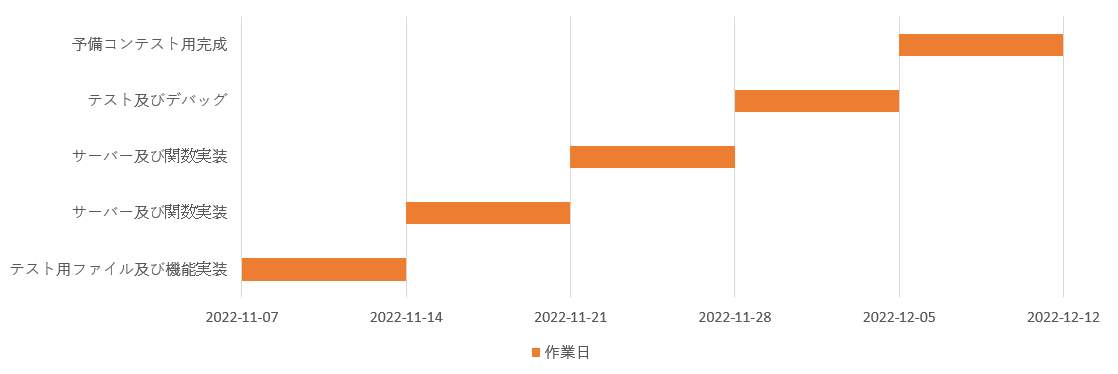
\includegraphics[scale=0.50]{gant.png}
	\caption{全員の開発ガントチャート}
	\label{fig:gc}
	\end{center}
	\end{figure}

\section{企画評価}
\subsection{技術}
\begin{table}[hbt]
	\begin{center}
	\caption{技術評価と理由}
	\label{table1}
	\begin{tabular}{|c|c|l|}\hline
	項目 & 評価値 & 理由 \\ \hline\hline
	ハードウェア構成 & 2 & Joyconを用いるため \\ \hline
	ゲームシステム & 2 & 物理演算及びイベント処理を追加 \\ \hline
	\end{tabular}
	\end{center}
	\end{table}
\subsection{企画}
\begin{table}[hbt]
	\begin{center}
	\caption{企画評価と理由}
	\label{table2}
	\begin{tabular}{|c|c|l|}\hline
	項目 & 評価値 & 理由 \\ \hline\hline
	オリジナリティ & 2 & ルールや目標が一緒があるかもしれないが達成方法が違うため \\ \hline
	面白さ・期待度 & 2 & 仲間と協力する分、達成感を一緒に味わえる\\ \hline
	\end{tabular}
	\end{center}
	\end{table}

\subsection{開発}
\begin{table}[hbt]
	\begin{center}
	\caption{企画評価と理由}
	\label{table3}
	\begin{tabular}{|c|c|l|}\hline
	項目 & 評価値 & 理由 \\ \hline\hline
	開発規模 & 2 & チャレンジするが開発に問題が内容調整予定 \\ \hline
	役割分担・開発計画 & 2 & 計画は前後する可能性があるが妥当に役割分担を行った \\ \hline
	受賞可能性 & 2 & マップとの相互作用・協力方式・プレイヤー経験を意識したため \\ \hline
	\end{tabular}
	\end{center}
	\end{table}

	\section{狙う賞}
	技術賞\\
	マップとの相互作用・物理演算などを理由とし\\
	技術賞を狙う。

	\section{アピールポイント}
	対戦型ではなく協力型で楽しめるものがある.\\
	このゲームは仲間と協力しその達成感を味わうように企画したため\\
	それを楽しんでほしい.


\end{document}